% Created 2017-09-26 Tue 19:25
% Intended LaTeX compiler: pdflatex
\documentclass[11pt]{article}
\usepackage[utf8]{inputenc}
\usepackage[T1]{fontenc}
\usepackage{graphicx}
\usepackage{grffile}
\usepackage{longtable}
\usepackage{wrapfig}
\usepackage{rotating}
\usepackage[normalem]{ulem}
\usepackage{amsmath}
\usepackage{textcomp}
\usepackage{amssymb}
\usepackage{capt-of}
\usepackage{hyperref}
\usepackage{minted}
\author{Kawin Nikomborirak}
\date{\today}
\title{}
\hypersetup{
 pdfauthor={Kawin Nikomborirak},
 pdftitle={},
 pdfkeywords={},
 pdfsubject={},
 pdfcreator={Emacs 25.3.1 (Org mode 9.1.1)}, 
 pdflang={English}}
\begin{document}

\tableofcontents

\begin{minted}[frame=single]{ipython}
%matplotlib inline
from modsim import *
\end{minted}

\begin{minted}[frame=single]{ipython}
system = System(t0=0,
		t_end=10,
		adult_pop0=10,
		birth_rate=0.9,
		death_rate=0.5,
		juvenile_pop0=0,
		mature_rate=0.33)

system
\end{minted}

\begin{minted}[frame=single]{ipython}
def run_simulation(system):
    """Runs a proportional growth model.

    Adds TimeSeries to `system` as `results`.

    system: System object with t0, t_end, p0,
	    birth_rate and death_rate
    """
    juveniles = TimeSeries()
    juveniles[system.t0] = system.juvenile_pop0
    adults = TimeSeries()
    adults[system.t0] = system.adult_pop0

    for t in linrange(system.t0, system.t_end):
	births = system.birth_rate * adults[t]
	deaths = system.death_rate * adults[t]
	maturations = juveniles[t] * system.mature_rate

	adults[t + 1] = adults[t] + maturations - deaths
	juveniles[t + 1] = juveniles[t] + births - maturations

    system.adults = adults
    system.juveniles = juveniles
\end{minted}

\begin{minted}[frame=single]{ipython}
run_simulation(system)
system.adults
\end{minted}

\begin{minted}[frame=single]{ipython}
def plot_results(system, title=None):
    """Plot the estimates and the model.

    system: System object with `results`
    """
    newfig()
    plot(system.adults, 'bo-', label='adults')
    plot(system.juveniles, 'rs-', label='juveniles')
    decorate(xlabel='Season',
	     ylabel='Rabbit population',
	     title=title)
\end{minted}

\begin{minted}[frame=single]{ipython}
plot_results(system, title='Proportional growth model')
\end{minted}

\begin{center}
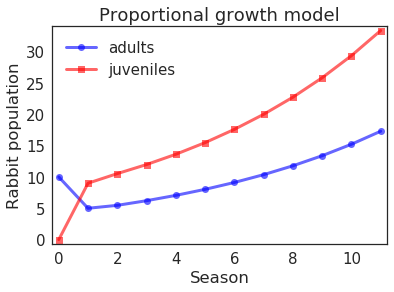
\includegraphics[width=.9\linewidth]{rab2fig/rabs.png}
\end{center}
\end{document}